\documentclass[11pt,twoside]{article}

\usepackage[margin=1in]{geometry}
\usepackage{amsmath,amssymb,amsthm,mathtools}
\usepackage{thmtools}
\usepackage[inline,shortlabels]{enumitem}
\usepackage{booktabs}
\usepackage{needspace}
\usepackage{tikz}
\usetikzlibrary{arrows.meta,positioning}
\usepackage{xcolor}
\usepackage{microtype}

% Revision date: maintained by scripts/build_lecture_notes.py. Keep this command.
\newcommand{\lecturerevised}{2026-10-03 01:15 UTC-06:00}
\usepackage{eso-pic}
\AddToShipoutPictureBG{%
  \AtPageLowerLeft{%
    \put(\LenToUnit{0.5\paperwidth},\LenToUnit{0.5in}){%
      \makebox(0,0){\normalfont\footnotesize\color{black!60}Last revised: \lecturerevised}%
    }%
  }%
}

\usepackage[square,authoryear]{natbib}
\usepackage[colorlinks=true,linkcolor=blue!60!black,
  urlcolor=blue!60!black,citecolor=blue!60!black]{hyperref}
\usepackage[nameinlink,capitalize]{cleveref}
\crefname{exercise}{Exercise}{Exercises}
\Crefname{exercise}{Exercise}{Exercises}
\hypersetup{pdftitle={Lecture 8: The need for signal},
  pdfauthor={Csaba Szepesvari}}

\usepackage{../exercises/course-exercises}
\newcommand{\suppmark}{\texorpdfstring{\textsuperscript{*}}{*}}

\usepackage{enotez}
\DeclareInstance{enotez-list}{lecture}{list}{format=\normalsize,number={#1.}}
\setenotez{list-name=Endnotes,list-style=lecture,backref=true}
\crefname{endnote}{Endnote}{Endnotes}
\Crefname{endnote}{Endnote}{Endnotes}

\definecolor{courseblue}{HTML}{17365D}
\newcommand{\E}{\mathbb E}
\newcommand{\I}{\mathbb I}
\renewcommand{\P}{\mathbb P}
\newcommand{\Law}{\mathcal L}
\newcommand{\R}{\mathbb R}
\newcommand{\KL}{D}
\newcommand{\TV}{\mathrm{TV}}
\makeatletter
\@for\@letter:=A,B,C,D,E,F,G,H,I,J,K,L,M,N,O,P,Q,R,S,T,U,V,W,X,Y,Z\do{%
  \expandafter\edef\csname c\@letter\endcsname{\noexpand\mathcal{\@letter}}}
\makeatother

\newtheorem{theorem}{Theorem}[section]
\newtheorem{proposition}[theorem]{Proposition}
\newtheorem{corollary}[theorem]{Corollary}
\newtheorem{lemma}[theorem]{Lemma}
\theoremstyle{definition}
\newtheorem{definition}[theorem]{Definition}
\newtheorem{example}[theorem]{Example}
\theoremstyle{remark}
\newtheorem{remark}[theorem]{Remark}

\renewcommand{\thepage}{8--\arabic{page}}
\renewcommand{\thesection}{8.\arabic{section}}
\renewcommand{\theequation}{8.\arabic{equation}}
\pagestyle{myheadings}
\markboth{Lecture 8: The need for signal}
{Lecture 8: The need for signal}

\begin{document}

\begin{center}
\fcolorbox{courseblue}{white}{%
\begin{minipage}{0.92\textwidth}
\vspace{1mm}
\textbf{CMPUT 654: Mathematical Foundations of Modern AI Systems}
\hfill Fall 2026

\vspace{3mm}
\begin{center}
{\Large\bfseries Lecture 8: The need for signal}

\vspace{1mm}
September 29, 2026
\end{center}

\vspace{2mm}
\textit{Lecturer: Csaba Szepesv\'ari}
\hfill
\textit{Note prepared by: Csaba Szepesv\'ari}
\vspace{1mm}
\end{minipage}}
\end{center}

\noindent\textbf{Reading guide.}
Lecture 7 gave an example in which a small ReLU network represents a fixed
parity but direct perturbed population-gradient training has no reliable
classification advantage. This lecture first proves that result. It then
changes the supervised task: running-parity labels expose a repeated two-bit
calculation whose final output is still the original parity. The path-star
example and a constructed transformer theorem show that retrieval and
combination must also be learned. The transformer theorem is included as
optional reading because its assumptions and three-update proof are useful for
understanding the mechanism but are not needed for the parity lower bound.
The prerequisites are Gaussian vectors, KL divergence, total variation,
Pinsker's inequality, Hoeffding's inequality, ReLU networks, and the parity
setup recalled below.

\section{The fixed-parity result}
\label{sec:recap}

Let $d\in\mathbb N$ and $[d]=\{1,\ldots,d\}$. For fixed $S\subseteq[d]$, write
\[
\chi_S(x)=\prod_{j\in S}x_j,
\qquad x\in\{-1,1\}^d.
\]
Let $X$ be uniform on $\{-1,1\}^d$, set $Y=\chi_S(X)$, and write $k=|S|$.

A one-hidden-layer ReLU network with $m\in\mathbb N$ units has parameter
\[
\theta=(u_r,w_r,b_r)_{r=1}^m\in\R^p,
\qquad u_r,b_r\in\R,\quad w_r\in\R^d,\quad p=m(d+2).
\]
We identify this tuple with the vector formed by concatenating its
coordinates. Write $[a]_+=\max\{a,0\}$, use $\|\cdot\|$ for the Euclidean
norm, and let $I_p$ denote the $p\times p$ identity matrix.
The network $N_\theta:\{-1,1\}^d\to\R$ and its signed correlation objective
$F:\R^p\to\R$ are
\begin{equation}
N_\theta(x)=\sum_{r=1}^m u_r[w_r^\top x+b_r]_+
\label{eq:relu-network}
\end{equation}
and
\begin{equation}
F(\theta)=-\E[Y N_\theta(X)].
\label{eq:correlation-objective}
\end{equation}
Lecture 7 constructed a width-$(k+1)$ network representing $\chi_S$. Thus
the lower bound below concerns optimization rather than representability.

For fixed $\theta$, define the classifier and its risk by
\[
h_\theta(x)=\operatorname{sign}(N_\theta(x)),
\qquad
R_{01}(h_\theta)=\P(h_\theta(X)\ne Y),
\]
where $\operatorname{sign}(0)=1$.\endnote{Zero network outputs.
Gaussian parameters can give the network output positive probability of being
zero. For each fixed $x$, the $m$ independent centered Gaussian margins are
all negative with probability $2^{-m}$; on that event every ReLU is zero.
The proof of \cref{thm:classification} works with either fixed binary value
for $\operatorname{sign}(0)$.}\label{en:zero-output}

Fix a number of updates $T\in\mathbb N$, a learning rate $\eta>0$, and a
noise scale $\sigma>0$. Let the
$\R^p$-valued random vectors $\Theta_0,\Xi_0,\ldots,\Xi_{T-1}$ be mutually
independent and independent of $X$, with
\[
\Law(\Theta_0)=\cN(0,\sigma^2I_p),
\qquad
\Law(\Xi_t)=\cN(0,\sigma^2I_p),\qquad 0\le t<T.
\]
Use the ReLU backpropagation rule $a\mapsto\I\{a>0\}$ in the updates.
The trained process and its gradient-free comparison process are
\begin{align}
\Theta_{t+1}&=\Theta_t-\eta\nabla F(\Theta_t)-\Xi_t,
\label{eq:perturbed-gd}\\
\Theta^{(0)}_0&=\Theta_0,
\qquad
\Theta^{(0)}_{t+1}=\Theta^{(0)}_t-\Xi_t.
\label{eq:gaussian-walk}
\end{align}

The following lemma compares the complete parameter trajectories. Its bound
will let us transfer a classification-risk calculation for the Gaussian walk
to the trained network.

\begin{restatable}[Path comparison]{lemma}{pathcomparison}
\label{lem:path-comparison}
Let $d>30$, $A>0$, $m,T\in\mathbb N$, and $\eta,\sigma>0$. Assume
\begin{equation}
m,T,\eta,\sigma,\sigma^{-1}\le d^A,
\qquad
k\ge(288A+144)\log d.
\label{eq:hardness-conditions}
\end{equation}
Then
\begin{equation}
\TV\!\left(
\Law(\Theta_0,\ldots,\Theta_T),
\Law(\Theta^{(0)}_0,\ldots,\Theta^{(0)}_T)
\right)
\le e^{-k/36}.
\label{eq:path-tv}
\end{equation}
\end{restatable}

The Gaussian walk is symmetric under changes of sign of individual parameter
coordinates. Combining that symmetry with the path comparison gives the
classification conclusion.

\begin{theorem}[Classification advantage occurs with probability at most one half]
\label{thm:classification}
Under the assumptions of \cref{lem:path-comparison}, for every $\gamma>0$,
\begin{align}
\P\!\left(R_{01}(h_{\Theta_T})\le\frac12-\gamma\right)
&\le\frac12+e^{-k/36},
\label{eq:classification-probability}\\
\left|\E[R_{01}(h_{\Theta_T})]-\frac12\right|
&\le e^{-k/36}.
\label{eq:classification-expectation}
\end{align}
\end{theorem}

\begin{proof}
By \cref{lem:path-comparison}, it suffices to establish the two risk bounds
for the Gaussian comparison parameter $G=\Theta_T^{(0)}$, with the
$e^{-k/36}$ terms removed. We will show that $R_{01}(h_G)$ and
$1-R_{01}(h_G)$ have the same law.

Fix $j\in S$. Let $D_j:\R^d\to\R^d$ flip the $j$th sign:
\[
D_j(x_1,\ldots,x_d)
=(x_1,\ldots,x_{j-1},-x_j,x_{j+1},\ldots,x_d).
\]
Define the corresponding parameter map by
\[
J_j:\R^p\to\R^p,\qquad
J_j\theta=(u_r,D_jw_r,b_r)_{r=1}^m.
\]
Both maps are orthogonal involutions:
$D_j^\top D_j=D_j^2=I_d$ and $J_j^\top J_j=J_j^2=I_p$.
The identities $(D_jw_r)^\top x=w_r^\top D_jx$ and $j\in S$ give
\[
N_{J_j\theta}(x)=N_\theta(D_jx),
\qquad
\chi_S(D_jx)=-\chi_S(x).
\]
Changing variables $z=D_jx$ in the uniform input average gives
\begin{align*}
R_{01}(h_{J_j\theta})
&=2^{-d}\sum_x\I\{h_\theta(D_jx)\ne\chi_S(x)\}\\
&=2^{-d}\sum_z\I\{h_\theta(z)\ne-\chi_S(z)\}
=1-R_{01}(h_\theta).
\end{align*}
Since $\Law(G)=\cN(0,(T+1)\sigma^2I_p)$ and $J_j$ is orthogonal,
$\Law(J_jG)=\Law(G)$.
Combining this invariance with the risk identity gives
\[
\Law(R_{01}(h_G))
=\Law(R_{01}(h_{J_jG}))
=\Law(1-R_{01}(h_G)).
\]
Thus the classification-risk distribution is symmetric about $1/2$. Hence
\[
\E[R_{01}(h_G)]=\frac12,
\qquad
\P\!\left(R_{01}(h_G)\le\frac12-\gamma\right)
=\P\!\left(R_{01}(h_G)\ge\frac12+\gamma\right)\le\frac12.
\]
The last inequality holds because the two events are disjoint.
Total variation controls the difference of event probabilities and of
expectations of $[0,1]$-valued functions. Applying \cref{eq:path-tv} to these
functions of the final parameter proves both conclusions.
\end{proof}

\section{Proof of the parity hardness result}
\label{sec:parity-proof}

It remains to prove the trajectory comparison in \cref{lem:path-comparison}.
The key estimate is an expected gradient bound under a Gaussian parameter
law. We first use this estimate to compare the trajectories, then prove it
by reducing the gradient coordinates to threshold correlations.

\begin{restatable}[Gaussian gradient]{lemma}{gaussiangradient}
\label{lem:gaussian-gradient}
Let $\Theta=(U_r,W_r,B_r)_{r=1}^m$ have independent
$\cN(0,\tau^2)$ coordinates, with $\tau>0$. If $d>30$ and $k\ge3$, then
\begin{equation}
\E[\|\nabla F(\Theta)\|]\le8md\tau e^{-k/8}.
\label{eq:gaussian-gradient-general}
\end{equation}
In particular, if $k\ge72\log(8md\tau)$, then
\begin{equation}
\E[\|\nabla F(\Theta)\|]\le e^{-k/9},
\label{eq:expected-gradient}
\end{equation}
and
\begin{equation}
\P(\|\nabla F(\Theta)\|\ge e^{-k/18})\le e^{-k/18}.
\label{eq:gradient-tail}
\end{equation}
\end{restatable}

\subsection{From small Gaussian gradients to close trajectories}

We use the Gaussian gradient estimate to prove the path comparison, restated
here with its parameter conditions.
\pathcomparison*

\begin{proof}[Proof of \cref{lem:path-comparison}]
We want to bound the total variation between the trained trajectory and the
Gaussian walk. Introduce a process that agrees with the Gaussian walk
whenever its gradient is small. For $\varepsilon=e^{-k/18}$, set
\begin{equation}
\overline\Theta_0=\Theta_0,
\qquad
\overline\Theta_{t+1}
=\overline\Theta_t-\eta[\nabla F(\overline\Theta_t)]_\varepsilon-\Xi_t,
\qquad
[g]_\varepsilon=
\begin{cases}
0,&\|g\|\le\varepsilon,\\
g,&\|g\|>\varepsilon.
\end{cases}
\label{eq:clipped-process}
\end{equation}
For any process $V_0,\ldots,V_T$, write $V_{0:T}=(V_0,\ldots,V_T)$.
Name the three \emph{trajectory laws}
\[
\mathsf P=\Law(\Theta_{0:T}),
\qquad
\mathsf R=\Law(\overline\Theta_{0:T}),
\qquad
\mathsf G=\Law(\Theta^{(0)}_{0:T}).
\]
The triangle inequality gives the two quantities to control:
\begin{equation}
\TV(\mathsf P,\mathsf G)
\le\TV(\mathsf P,\mathsf R)+\TV(\mathsf R,\mathsf G).
\label{eq:path-triangle}
\end{equation}

\paragraph{The trained and auxiliary processes have close transition laws.}
We bound $\TV(\mathsf P,\mathsf R)$ through KL. For a history
$\vartheta_{0:t}\in(\R^p)^{t+1}$, the recursions specify the following
versions of their next-step conditional laws:
\begin{align*}
\mathsf P_t(\,\cdot\mid\vartheta_{0:t})
&=\Law(\Theta_{t+1}\mid\Theta_{0:t}=\vartheta_{0:t})\\
&=\cN\bigl(\vartheta_t-\eta\nabla F(\vartheta_t),\sigma^2I_p\bigr),\\
\mathsf R_t(\,\cdot\mid\vartheta_{0:t})
&=\Law(\overline\Theta_{t+1}\mid
             \overline\Theta_{0:t}=\vartheta_{0:t})\\
&=\cN\bigl(\vartheta_t-\eta[\nabla F(\vartheta_t)]_\varepsilon,
             \sigma^2I_p\bigr).
\end{align*}
These formulas define kernels from $(\R^p)^{t+1}$ to probability laws on
$\R^p$. At the same history, their means differ by
\[
\eta\bigl(\nabla F(\vartheta_t)-[\nabla F(\vartheta_t)]_\varepsilon\bigr),
\]
whose norm is at most $\eta\varepsilon$. The KL formula for Gaussians with
the same covariance gives
\[
\KL\bigl(\mathsf P_t(\,\cdot\mid\vartheta_{0:t}),
\mathsf R_t(\,\cdot\mid\vartheta_{0:t})\bigr)
=\frac{\eta^2}{2\sigma^2}
\bigl\|\nabla F(\vartheta_t)-[\nabla F(\vartheta_t)]_\varepsilon\bigr\|^2
\le\frac{\eta^2\varepsilon^2}{2\sigma^2}.
\]
The initial laws agree. Thus the KL chain rule gives
\begin{align}
\KL(\mathsf P,\mathsf R)
&=\sum_{t=0}^{T-1}\E_{\mathsf P}\!\left[
\KL\bigl(\mathsf P_t(\,\cdot\mid\Theta_{0:t})
,\mathsf R_t(\,\cdot\mid\Theta_{0:t})\bigr)\right]
\le\frac{T\eta^2\varepsilon^2}{2\sigma^2}.
\label{eq:path-kl}
\end{align}
By Pinsker's inequality,
\begin{equation}
\TV(\mathsf P,\mathsf R)
\le\sqrt{\frac12\KL(\mathsf P,\mathsf R)}
\le\frac{\eta\varepsilon\sqrt T}{2\sigma}.
\label{eq:actual-aux-tv}
\end{equation}

\paragraph{The auxiliary process agrees with the Gaussian walk with high probability.}
Use the same initialization and increments for both processes, as in
\cref{eq:gaussian-walk,eq:clipped-process}. On the event
\[
E=\left\{\max_{0\le t\le T}\|\nabla F(\Theta_t^{(0)})\|
\le\varepsilon\right\},
\]
their trajectories coincide. Indeed, if
$\overline\Theta_t=\Theta_t^{(0)}$, then the auxiliary gradient is zero and
both recursions subtract $\Xi_t$. Induction proves equality at every time
on $E$. The coupling inequality therefore gives
\[
\TV(\mathsf R,\mathsf G)\le\P(E^c).
\]

To bound $\P(E^c)$, we apply \cref{lem:gaussian-gradient} at each time.
The independent Gaussian increments give
\[
\Law(\Theta_t^{(0)})=\cN(0,(t+1)\sigma^2I_p),
\qquad \tau_t=\sigma\sqrt{t+1}.
\]
The parameter conditions in \cref{eq:hardness-conditions} imply, for $t\le T$,
\begin{align*}
\log(8md\tau_t)
&\le\log(8\sqrt2)+(1+5A/2)\log d
\le(4A+2)\log d
\le k/72.
\end{align*}
Here we used $m,\sigma,T\le d^A$ and $d>30$; the lower bound on $k$ also
implies $k\ge3$. Thus the Gaussian gradient estimate applies and gives
\[
\E[\|\nabla F(\Theta_t^{(0)})\|]\le e^{-k/9}=\varepsilon^2,
\qquad
\P(\|\nabla F(\Theta_t^{(0)})\|>\varepsilon)\le\varepsilon
\]
by Markov's inequality. A union bound now yields
\begin{equation}
\P(E^c)
=\P\!\left(\max_{0\le t\le T}\|\nabla F(\Theta_t^{(0)})\|
>\varepsilon\right)
\le(T+1)\varepsilon,
\label{eq:walk-good-event}
\end{equation}
so
\begin{equation}
\TV(\mathsf R,\mathsf G)\le(T+1)\varepsilon.
\label{eq:aux-walk-tv}
\end{equation}

\paragraph{Combining the two comparisons.}
Substituting \cref{eq:actual-aux-tv,eq:aux-walk-tv} into
\cref{eq:path-triangle} gives
\begin{equation}
\TV(\mathsf P,\mathsf G)
\le\left(\frac{\eta\sqrt T}{2\sigma}+T+1\right)e^{-k/18}.
\label{eq:complete-path-bound}
\end{equation}
The polynomial bounds on $\eta,T,\sigma^{-1}$ give
\[
\frac{\eta\sqrt T}{2\sigma}+T+1\le3d^{5A/2}.
\]
Finally,
\[
\log(3d^{5A/2})
=\log3+\frac{5A}{2}\log d
\le(8A+4)\log d
\le k/36.
\]
Consequently, \cref{eq:complete-path-bound} is at most
$e^{k/36}e^{-k/18}=e^{-k/36}$, as claimed.
\end{proof}

\subsection{Bounding the expected gradient one unit at a time}
\label{sec:gaussian-gradient-proof}

The path argument used the following estimate at variance
$\tau^2=(t+1)\sigma^2$. We now prove it for any $\tau>0$.
\gaussiangradient*

\begin{proof}[Proof of \cref{lem:gaussian-gradient}]
We need to bound $\E[\|\nabla F(\Theta)\|]$.
We start by calculating the derivative of $F$ at some fixed parameter vector $\theta\in \R^p$.
Grouping the derivatives by hidden unit gives
\begin{align}
\|\nabla F(\theta)\|
=\sqrt{\sum_{r=1}^m\left(
|\partial_{u_r}F(\theta)|^2+
\|\partial_{w_r}F(\theta)\|^2+
|\partial_{b_r}F(\theta)|^2\right)}.
\label{eq:enabft}
\end{align}
We now turn to calculating the derivatives appearing in this expression.
For this, let $X$ be independent of $\Theta$, with
$\Law(X)=\operatorname{Unif}(\{-1,1\}^d)$.

For fixed $\theta$, the objective in \cref{eq:correlation-objective} is
$F(\theta)=-\E[\chi_S(X)N_\theta(X)]$.
Differentiating this finite average and using
that for every
$x\in\{-1,1\}^d$,
\[
x_i\chi_S(x)=\chi_{S\mathbin\triangle\{i\}}(x)
\]
we get
\begin{align}
\partial_{u_r}F(\theta)
&=-\E[\chi_S(X)[w_r^\top X+b_r]_+],
\label{eq:u-derivative}\\
\partial_{b_r}F(\theta)
&=-u_rq_S(w_r,b_r),
\label{eq:b-derivative}\\
\partial_{w_{r,i}}F(\theta)
&=-u_rq_{S\mathbin\triangle\{i\}}(w_r,b_r).
\label{eq:w-derivative}
\end{align}
where
for $B\subseteq[d]$,
the function $q_B: \R^d\times \R \to \R$ is defined by
\begin{equation}
q_B(w,b)=\E[\chi_B(X)\I\{w^\top X+b>0\}]\,, \quad w\in \R^d, b\in \R\,.
\label{eq:threshold-coefficient}
\end{equation}
The identities stated for the
derivatives hold whenever the preactivation margins are nonzero, which
occurs almost surely at Gaussian parameters.

We now show that the output-weight derivative
also reduces to threshold correlations: since $[z]_+=z\I\{z>0\}$,
\begin{align}
\partial_{u_r}F(\theta)
&=-\E[\chi_S(X)(w_r^\top X+b_r)
                 \I\{w_r^\top X+b_r>0\}]\notag\\
&=-b_rq_S(w_r,b_r)
-\sum_{i=1}^dw_{r,i}q_{S\mathbin\triangle\{i\}}(w_r,b_r).
\label{eq:u-expansion}
\end{align}


We now return to bounding $\E[\|\nabla F(\Theta)\|]$.
Plugging $\Theta$ into \cref{eq:enabft},
repeatedly applying $\sqrt{x+y}\le\sqrt x+\sqrt y$,
and then taking expectation of both sides,
then applying Jensen's to move the expectation under the remaining
square roots yields
\begin{equation}
\E[\|\nabla F(\Theta)\|]
\le\sum_{r=1}^m\left(
\E[|\partial_{u_r}F(\Theta)|]
+\sqrt{\E[\|\partial_{w_r}F(\Theta)\|^2]
+\E[|\partial_{b_r}F(\Theta)|^2]}
\right).
\label{eq:gradient-decomposition}
\end{equation}
From our earlier expression for the partial derivatives with respect to
the first layer parameters $(w_r,b_r)$ we see that we will need bounds on the
expected value of $q_B(W_r,B_r)^2$. The reason the partial derivative
with respect to $u_r$ is treated differently will become clear momentarily.

\cref{lem:gaussian-threshold}, stated and proved below, gives
\[
\E[q_B(W_r,B_r)^2]\le8e^{-|B|/4}.
\]
Because $|S|=k$ and $|S\mathbin\triangle\{i\}|\ge k-1\ge2$, this inequality gives
\[
\E[q_S(W_r,B_r)^2]\le8e^{-k/4},
\qquad
\E[q_{S\mathbin\triangle\{i\}}(W_r,B_r)^2]
\le8e^{-(k-1)/4}<11e^{-k/4}.
\]
% We now use these two estimates in \cref{eq:gradient-decomposition}.
For the output-weight term, \cref{eq:u-expansion} and Cauchy--Schwarz give
\begin{align}
\E[|\partial_{u_r}F(\Theta)|]
&\le\sqrt{\E[B_r^2]\E[q_S(W_r,B_r)^2]}
+\sqrt{\E[\|W_r\|^2]\,
\E\!\left[\sum_{i=1}^dq_{S\mathbin\triangle\{i\}}(W_r,B_r)^2\right]}
\notag\\
&\le\sqrt8\,\tau e^{-k/8}+\sqrt{11}\,d\tau e^{-k/8}
\le7d\tau e^{-k/8}.
\label{eq:u-coordinate-bound}
\end{align}
For the input weights and bias, $U_r$ is independent of $(W_r,B_r)$.
Thus \cref{eq:b-derivative,eq:w-derivative} give
\begin{align}
\E[|\partial_{b_r}F(\Theta)|^2]
&=\E[U_r^2]\E[q_S(W_r,B_r)^2]
\le8\tau^2e^{-k/4},
\label{eq:b-coordinate-bound}\\
\E[\|\partial_{w_r}F(\Theta)\|^2]
&=\tau^2\sum_{i=1}^d
\E[q_{S\mathbin\triangle\{i\}}(W_r,B_r)^2]
\le11d\tau^2e^{-k/4}.
\label{eq:w-coordinate-bound}
\end{align}
Substituting these bounds into \cref{eq:gradient-decomposition} proves
\[
\E[\|\nabla F(\Theta)\|]
\le m\tau e^{-k/8}(7d+\sqrt{11d+8})
\le8md\tau e^{-k/8},
\]
where $d>30$ ensures the last inequality. If
$k\ge72\log(8md\tau)$, then $8md\tau\le e^{k/72}$ and the bound becomes
$e^{-k/9}$. Markov's inequality at threshold $e^{-k/18}$ proves
\cref{eq:gradient-tail}.
\end{proof}

\subsection{Why a Gaussian threshold has little correlation with parity}

It remains to bound the threshold coefficients used in the gradient proof.
Averaging their squares over Gaussian parameters will turn the calculation
into a polynomial expansion on the Boolean cube. Every power of degree below
$|B|$ cancels.

\begin{lemma}[Gaussian threshold correlation]
\label{lem:gaussian-threshold}
Let $(W,C)$ have law $\cN(0,\tau^2I_{d+1})$, with $\tau>0$.
For every $B\subseteq[d]$ with $|B|\ge2$,
\begin{equation}
\E[q_B(W,C)^2]\le8e^{-|B|/4}.
\label{eq:threshold-bound}
\end{equation}
\end{lemma}

\begin{proof}
To evaluate $\E[q_B(W,C)^2]$, expand the two copies of the input average.
Let $X,X'$ be independent uniform random vectors in $\{-1,1\}^d$,
independent of $(W,C)$. All probabilities and expectations in this proof
refer to this joint experiment. Then
\[
\E[q_B(W,C)^2]
=\E\!\left[\chi_B(X)\chi_B(X')
\P(W^\top X+C>0,\ W^\top X'+C>0\mid X,X')\right].
\]
For $x,x'\in \R^d$ fixed, $W^\top x+C, W^\top x'+C$
are centered Gaussian variables with
common variance $\tau^2(d+1)$ and covariance $\tau^2(x^\top x'+1)$. Their
correlation is therefore $(x^\top x'+1)/(d+1)$. The Gaussian orthant formula
gives
\begin{equation}
\E[q_B(W,C)^2]
=\E\!\left[\chi_B(X)\chi_B(X')
\left(\frac14+\frac1{2\pi}\arcsin\frac{X^\top X'+1}{d+1}\right)\right].
\label{eq:orthant-expansion}
\end{equation}
Set $Z_i=X_iX'_i$ and $V=(1+\sum_iZ_i)/(d+1)$. The $Z_i$ are independent
uniform signs, $\chi_B(X)\chi_B(X')=\chi_B(Z)$, and
$\E[\chi_B(Z)]=0$. Hence
\[
\E[q_B(W,C)^2]=\frac1{2\pi}\E[\chi_B(Z)\arcsin V].
\]

To bound this expression, we use the Taylor expansion
\[
\arcsin v=\sum_{\ell\ge0}a_\ell v^\ell,
\qquad |v|\le1,\qquad
a_\ell\ge0,\qquad \sum_{\ell\ge0}a_\ell=\frac\pi2.
\]
The series converges absolutely and uniformly on $[-1,1]$;
\cref{app:arcsine-series} gives the coefficients and proves these properties.
Absolute summability justifies exchanging the series and expectation, giving
\[
\E[q_B(W,C)^2]
=\frac1{2\pi}\sum_{\ell\ge0}a_\ell\E[\chi_B(Z)V^\ell].
\]
We first eliminate every term of degree $\ell<|B|$. Expanding
$(1+\sum_i Z_i)^\ell$, each monomial \textbf{omits} at least one coordinate in $B$.
Averaging over that independent mean-zero sign gives
\begin{equation}
\E[\chi_B(Z)V^\ell]=0,\qquad \ell<|B|.
\label{eq:degree-cancellation}
\end{equation}
Since $|V|\le1$, for the remaining terms
with $\ell \ge |B|$ we have $|V|^\ell \le |V|^{|B|}$ and hence
\begin{align*}
\E[q_B(W,C)^2]
&\le\frac1{2\pi}\sum_{\ell\ge|B|}a_\ell\E[|V|^\ell]
\le\frac14\E[|V|^{|B|}].
\end{align*}

We now bound this single moment. Hoeffding's inequality gives
\[
\P\!\left(\left|\sum_{i=1}^dZ_i\right|>\frac{3d}{4}\right)
\le2e^{-9d/32}.
\]
On the complementary event,
\[
|V|\le\frac{3d/4+1}{d+1}
=\frac34\left(1+\frac1{3(d+1)}\right)
\le \frac34 \exp(\frac1{3(d+1)})\,,
\]
where the last inequality used that $1+t \le e^t$.
Raising this bound to power $|B|$ and using $|B|\le d+1$ gives
$|V|^{|B|}\le e^{1/3}(3/4)^{|B|}$. Using $|V|\le1$ on the exceptional
event, we conclude that
\[
\E[q_B(W,C)^2]
\le\frac14\left(2e^{-9d/32}+e^{1/3}(3/4)^{|B|}\right)
\le8e^{-|B|/4},
\]
where the last inequality uses $d\ge|B|$, $9/32>1/4$, and
$\log(4/3)>1/4$.
\end{proof}

On the Boolean cube, the functions $\chi_B$ form the \emph{Fourier character}
basis. The character $\chi_B$ has degree $|B|$. Thus
\cref{eq:degree-cancellation} says that every polynomial of degree below
$|B|$ has zero coefficient in the $\chi_B$ direction. This cancellation
leaves only high powers of $V$, whose moments are exponentially small.
The scale $\tau$ disappears because multiplying $(W,C)$ by a positive number
does not change the threshold.\endnote{General activations.
\Cref{ex:l8-activation-generalization} asks you to extend the lower bound
using the nonnegative series coefficients of Gaussian activation kernels,
parity cancellation, and bounds on Gaussian second moments.}
\label{en:general-activations}

\section{Intermediate labels expose a repeated two-bit computation}
\label{sec:intermediate}

The lower bound applies to direct training on the final parity label. To change
the supervised task while preserving its final answer, write
$x_i=(-1)^{b_i}$ with $b_i\in\{0,1\}$ and define
\begin{equation}
z_1=b_1,
\qquad
z_i=z_{i-1}\oplus b_i,
\qquad 2\le i\le d.
\label{eq:running-parity}
\end{equation}
Then $(-1)^{z_d}=\chi_{[d]}(x)$. Supplying
$z_1,\ldots,z_d$ during training gives a label for every application of the
same local rule. The following proposition gives that rule explicitly and
verifies that composing it solves the original parity task.

\begin{proposition}[A local XOR rule composes into parity]
\label{prop:xor-compose}
The function
\[
g(a,b)=[a+b]_+-2[a+b-1]_++[a+b-2]_+
\]
equals $a\oplus b$ on $\{0,1\}^2$. If
$\widehat z_1=b_1$ and
$\widehat z_i=g(\widehat z_{i-1},b_i)$, then
\[
\widehat z_i=b_1\oplus\cdots\oplus b_i
\]
for every $i$. In particular,
$(-1)^{\widehat z_d}=\chi_{[d]}(x)$.
\end{proposition}

\begin{proof}
We prove the running-parity identity by induction. At $i=1$ it holds because
$\widehat z_1=b_1$. For the induction step, we need $g(a,b)=a\oplus b$
for binary $a,b$. Evaluating the ReLU expression at $a+b=0,1,2$ gives
$0,1,0$, respectively, which is exactly XOR. Thus, if the identity holds
at $i-1$, then
\[
\widehat z_i=g(\widehat z_{i-1},b_i)
=\widehat z_{i-1}\oplus b_i
=b_1\oplus\cdots\oplus b_i.
\]
Taking $i=d$ proves the final claim.
\end{proof}

One implementation can train a network for $g$ and then place copies of that
network in a prescribed computation graph. The connections are supplied by
the construction. A single sequence model has the harder job of learning both
the local rule and the routing that supplies its arguments.

Fix the predictors after training. The following proposition relates their
errors on correct prefixes to the errors made when their own predictions
are supplied as prefixes.

\begin{proposition}[Local errors control the probability of a rollout error]
\label{prop:rollout-union}
Let $(X,Z_{1:d})$ be a random input and target sequence taking values in
$\cX\times\cZ^d$, where $\cZ$ is a finite output alphabet. For fixed predictors
\[
g_i:\cX\times\cZ^{i-1}\to\cZ,\qquad i\in[d],
\]
define the rollout recursively by
\[
\widehat Z_i=g_i(X,\widehat Z_{<i}),\qquad i\in[d],
\]
where $Z_{<1}$ and $\widehat Z_{<1}$ are empty prefixes. Define the
\emph{teacher-forced error events}
\[
E_i=\{g_i(X,Z_{<i})\ne Z_i\},\qquad i\in[d].
\]
Then
\begin{equation}
\{\widehat Z_{1:d}\ne Z_{1:d}\}=\bigcup_{i=1}^dE_i.
\label{eq:rollout-error-event}
\end{equation}
Consequently,
\[
\P(\widehat Z_d\ne Z_d)
\le\P(\widehat Z_{1:d}\ne Z_{1:d})
\le\sum_{i=1}^d\P(E_i).
\]
\end{proposition}

\begin{proof}
We characterize the event that the first $i$ predictions are all correct.
On $\{\widehat Z_{<i}=Z_{<i}\}$, the two evaluations of $g_i$ have the
same arguments. Hence
\[
\{\widehat Z_{1:i}=Z_{1:i}\}
=\{\widehat Z_{<i}=Z_{<i}\}\cap E_i^c.
\]
Starting with the empty prefix and applying this identity successively gives
\[
\{\widehat Z_{1:d}=Z_{1:d}\}=\bigcap_{i=1}^dE_i^c.
\]
Taking complements proves \cref{eq:rollout-error-event}. Finally,
$\{\widehat Z_d\ne Z_d\}\subseteq
\{\widehat Z_{1:d}\ne Z_{1:d}\}$, and the union bound gives the stated
probability inequalities.
\end{proof}

Thus $\P(E_i)\le\varepsilon$ for every $i$ gives a final-answer error
bound of $\min\{1,d\varepsilon\}$. To guarantee a final-answer error at
most $\delta$, it suffices to have
$\sum_i\P(E_i)\le\delta$; equal per-step bounds of $\delta/d$ are one
way to ensure this.

\section{The path-star task hides parity in its first decision}
\label{sec:path-star}

A path-star graph consists of several directed paths that share a center. An
example supplies the shuffled edge list, the center, a designated leaf, and
the center-to-leaf path. During forward teacher forcing, the model receives
the true preceding path token. Once the first edge has been chosen, each
internal node has a unique outgoing edge along its arm. A predictor can
therefore learn almost every next-token prediction while still guessing which
arm contains the goal.

The remaining first decision can encode full parity. Given bits
$b_1,\ldots,b_{q-1}$, use vertices
$-q,\ldots,-1,0,1,\ldots,q$. Connect $0$ to both $1$ and $-1$. For
$1\le i<q$, add
\[
\begin{array}{c|cc}
&\text{edge from }i&\text{edge from }-i\\
\hline
b_i=0&i\to i+1&-i\to-(i+1)\\
b_i=1&i\to-(i+1)&-i\to i+1.
\end{array}
\]
\Cref{fig:path-star} shows the construction for three bits. It also marks
the first branch that must be chosen to reach the designated goal.

\begin{figure}[htbp]
\centering
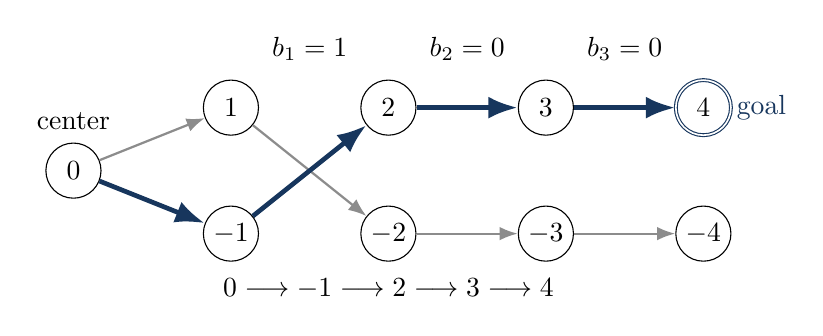
\begin{tikzpicture}[
  >=Latex, x=2cm, y=1cm,
  vertex/.style={circle,draw,fill=white,minimum size=7mm,inner sep=1pt},
  edge/.style={->,draw=black!45,line width=0.8pt},
  route/.style={->,draw=courseblue,line width=1.7pt}]
\node[vertex] (center) at (0,0) {$0$};
\foreach \i in {1,2,3,4}{
  \node[vertex] (p\i) at (\i,0.8) {$\i$};
  \node[vertex] (n\i) at (\i,-0.8) {$-\i$};
}
\draw[edge] (center)--(p1);
\draw[edge] (p1)--(n2);
\draw[edge] (n2)--(n3);
\draw[edge] (n3)--(n4);
\draw[route] (center)--(n1);
\draw[route] (n1)--(p2);
\draw[route] (p2)--(p3);
\draw[route] (p3)--(p4);
\node[vertex,draw=courseblue,double] at (p4) {$4$};
\node[above=4mm] at (center) {center};
\node[right=3mm,text=courseblue] at (p4) {goal};
\node at (1.5,1.55) {$b_1=1$};
\node at (2.5,1.55) {$b_2=0$};
\node at (3.5,1.55) {$b_3=0$};
\node at (2,-1.5) {$0\longrightarrow-1\longrightarrow2
                         \longrightarrow3\longrightarrow4$};
\end{tikzpicture}
\caption{The two-arm path-star for $(b_1,b_2,b_3)=(1,0,0)$.
The highlighted path reaches goal $4$. Since $1\oplus0\oplus0=1$, its
first vertex is $-1$. Each later step follows a unique outgoing edge.}
\label{fig:path-star}
\end{figure}

Each bit equal to one switches the sign of the current vertex. Therefore the
path that starts with $s\in\{-1,1\}$ reaches the leaf
$sq(-1)^{b_1+\cdots+b_{q-1}}$. To reach the goal $q$, its first step must be
\begin{equation}
\begin{cases}
1,&b_1\oplus\cdots\oplus b_{q-1}=0,\\
-1,&b_1\oplus\cdots\oplus b_{q-1}=1.
\end{cases}
\label{eq:path-star-parity}
\end{equation}
Predicting the correct first edge on every graph in this family computes full
parity. The example separates high average teacher-forced accuracy from
learning the decision needed to generate the correct path. Backward or
intermediate supervision reveals information about the goal arm before the
first forward decision.

\section{Optional reading: a constructed transformer learns retrieval and XOR}
\label{sec:transformer}

The composition in \cref{sec:intermediate} supplied the connections between
copies of the XOR rule. A sequence model must learn which input to retrieve
as well as how to combine it with the current state. The following
construction trains both components with intermediate labels. Its three
updates have distinct roles: create a retrieval signal, concentrate attention,
and fit the local output rule.

\paragraph{The supervised sequence.}
Keep $d$ for the number of input bits. Fix
\[
\cI=\{d+1,\ldots,d+k\},
\qquad s:\cI\to[d]\ \text{injective},
\qquad S=s(\cI).
\]
The teacher chooses $s$ and supplies sequences with the running parities
\begin{equation}
b_{d+1}=0,\qquad
b_{i+1}=b_i\oplus b_{s(i)},\quad i\in\cI.
\label{eq:subset-running-parity}
\end{equation}
Thus $b_{d+k+1}=\bigoplus_{j\in S}b_j$. Let
\[
\cB_s=\{b\in\{0,1\}^{d+k+1}:
b_{d+1}=0,\ b_{i+1}=b_i\oplus b_{s(i)}\text{ for all }i\in\cI\}.
\]
The training law $P_{\rm CoT}$ is the law of the random sequence
$\mathbf B=(B_1,\ldots,B_{d+k+1})$ obtained from independent uniform input
bits $B_1,\ldots,B_d$ and the recursion in
\cref{eq:subset-running-parity}. The student receives these sequences;
$s$ is learned from them.

At position $i$, the model receives the correct prefix $b_{1:i}$ and
predicts $b_{i+1}$. We use the signed label
\[
y_i(b)=2b_{i+1}-1\in\{-1,1\}.
\]
A positive prediction score represents bit $1$. Supplying the correct prefix
at each supervised position is \emph{teacher forcing}.

\paragraph{The model.}
Let $D\in\mathbb N$ be the embedding dimension and $m\in\mathbb N$ the
feed-forward width. For each position $i\in[d+k]$ and bit $a\in\{0,1\}$,
draw an independent
frozen embedding $e_{i,a}\in\R^D$ with
\[
\Law(e_{i,a})=\operatorname{Unif}
\bigl(\{-D^{-1/2},D^{-1/2}\}^D\bigr),
\qquad v_i(b)=e_{i,b_i}.
\]
The trainable attention matrix is $A\in\R^{D\times D}$. Its scores, causal
attention weights, and retrieved vector are
\begin{align}
s_{ji}(A;b)&=v_j(b)^\top A v_i(b),\notag\\
\alpha_{ji}(A;b)
&=\frac{\exp s_{ji}(A;b)}{\sum_{\ell=1}^i\exp s_{\ell i}(A;b)},
\quad 1\le j\le i,\notag\\
c_i(A;b)&=\sum_{j=1}^i\alpha_{ji}(A;b)v_j(b).
\label{eq:transformer-attention}
\end{align}
Set $\alpha_{ji}=0$ for $j>i$. The two arguments of the local computation
enter separate blocks of the feed-forward weight matrix:
\[
W=[W^{\rm tok}\ W^{\rm att}]\in\R^{m\times2D},
\qquad W^{\rm tok},W^{\rm att}\in\R^{m\times D}.
\]
With fixed $h\in\R^m$, the score at position $i$ is
\begin{equation}
f_{W,A}(b)_i
=h^\top\left[W
\begin{pmatrix}v_i(b)\\c_i(A;b)\end{pmatrix}\right]_+
=h^\top[W^{\rm tok}v_i(b)+W^{\rm att}c_i(A;b)]_+.
\label{eq:transformer-score}
\end{equation}
Here ReLU acts coordinatewise. Concatenation gives the feed-forward layer
separate access to the current token and the attention output.

\paragraph{Initialization and training.}
The initialization is designed so that the current token selects the ReLU
gates before attention contributes to the score. For an even width $m$ and
an amplitude $\epsilon>0$, set
\begin{align}
A^{(0)}&=0,\qquad (W^{\rm att})^{(0)}=0,\notag\\
(W^{\rm tok})^{(0)}_{r,:}
&=\sum_{i\in\cI}\sum_{a=0}^1\nu_{r,i,a}e_{i,a}^\top,\qquad
\Law(\nu_{r,i,a})=\operatorname{Unif}\{-\epsilon,\epsilon\},\notag\\
h_r&=
\begin{cases}
1/m,&1\le r\le m/2,\\
-1/m,&m/2<r\le m.
\end{cases}
\label{eq:transformer-initialization}
\end{align}
All $\nu_{r,i,a}$ are independent of one another and of the embeddings.
The embeddings and $h$ remain fixed. Both $W$ and $A$ are updated.

For one sequence, the \emph{hinge loss} summed over supervised positions is
\[
\ell(W,A;b)=\sum_{i\in\cI}\ell_i(W,A;b),
\qquad
\ell_i(W,A;b)=[1-y_i(b)f_{W,A}(b)_i]_+.
\]
For each $t=0,1,2$, draw a fresh batch of $n$ independent sequences
$\mathbf B^{(t,1)},\ldots,\mathbf B^{(t,n)}$ with law $P_{\rm CoT}$.
The three batches are mutually independent and independent of initialization.
With $\vartheta=(W,A)$, define
\begin{equation}
\widehat F_t(W,A)=\frac1n\sum_{a=1}^n\ell(W,A;\mathbf B^{(t,a)}),
\qquad
\vartheta^{(t+1)}
=\vartheta^{(t)}-\eta_t\nabla\widehat F_t(\vartheta^{(t)}).
\label{eq:transformer-updates}
\end{equation}
The gradient updates all entries of both matrices at each step.

The next result states parameter scales for which these three simultaneous
updates learn every supervised prediction and the required retrieval map.
All asymptotic statements concern sufficiently large $d$.

\Needspace{21\baselineskip}
\begin{theorem}[Three-update parity learning under structured initialization]
\label{thm:three-update}
Fix $\delta\in(0,1/2)$ and a sufficiently small constant $\epsilon>0$, and set
$\Lambda=\log(d/\delta)$. Suppose
\[
\frac{d}{\Lambda^5}\le k\le\frac{d}{\Lambda^4}.
\]
There are absolute constants $C_{\rm batch},c_{\rm init},c_{\rm final}>0$
such that the model, initialization, and updates in
\cref{eq:transformer-attention,eq:transformer-score,eq:transformer-initialization,eq:transformer-updates},
with
\begin{align*}
D&=\lceil k\Lambda^{11/10}\rceil,\qquad m=4k,\qquad
n=\lceil C_{\rm batch}\epsilon^{-2}d\Lambda^{20}\rceil,\\
\eta_0&=\eta_1=c_{\rm init}\frac{m\epsilon\sqrt n}{\Lambda},
\qquad \eta_2=c_{\rm final}k\epsilon,
\end{align*}
satisfy, with probability at least $1-\delta$,
\begin{equation}
\begin{gathered}
y_i(b)f_{W^{(3)},A^{(3)}}(b)_i>0,\\
\alpha_{s(i),i}(A^{(3)};b)\ge1-d^{-8}
\end{gathered}
\qquad
\text{for every }b\in\cB_s\text{ and }i\in\cI.
\label{eq:transformer-conclusions}
\end{equation}
The probability includes the random embeddings, initialization signs, and
three training batches.
\end{theorem}

The first inequality gives the correct next bit at every correct prefix.
Starting from the supplied input and $b_{d+1}=0$, induction therefore gives
the correct entire running-parity sequence during generation. All three
batches have the same sequence length $d+k+1$.

\begin{proof}[Proof outline]
We need to establish correct retrieval and a positive signed output at every
supervised position. The proof tracks these quantities through the three
updates. We give the gradient identities and the estimates that connect the
steps; the accompanying concentration arguments are in the source identified
in the bibliographical notes.

For fixed $b\in\cB_s$, abbreviate $v_i=v_i(b)$ and
$c_i^{(t)}=c_i(A^{(t)};b)$. Define the preactivation of unit $r$ by
\[
\rho_{r,i}^{(t)}(b)
=\bigl((W^{\rm tok})^{(t)}v_i
       +(W^{\rm att})^{(t)}c_i^{(t)}\bigr)_r.
\]
We will use the diagonal gate matrix
\[
\Gamma_{i,a}=\operatorname{diag}
\bigl(\I\{\nu_{r,i,a}>0\}:r\in[m]\bigr).
\]

\paragraph{First update: the feed-forward weights acquire a retrieval signal.}
At initialization, $A^{(0)}=0$ gives uniform attention:
\[
\alpha_{ji}(A^{(0)};b)=\frac1i,
\qquad
c_i^{(0)}=\frac1i\sum_{j=1}^i v_j.
\]
The initialization separates the matching embedding from the remaining terms:
\[
\rho_{r,i}^{(0)}(b)
=\nu_{r,i,b_i}
+\sum_{\substack{j\in\cI,\ a\in\{0,1\}\\(j,a)\ne(i,b_i)}}
\nu_{r,j,a}\langle e_{j,a},e_{i,b_i}\rangle.
\]
Concentration of the random sum gives, with high probability,
\[
|\rho_{r,i}^{(0)}(b)-\nu_{r,i,b_i}|\le\epsilon/4
\quad\Longrightarrow\quad
\I\{\rho_{r,i}^{(0)}(b)>0\}=\I\{\nu_{r,i,b_i}>0\}.
\]
Thus the gates are $\Gamma_{i,b_i}$. Since $(W^{\rm att})^{(0)}=0$, the
chain rule gives
\[
\nabla_A\widehat F_0(W^{(0)},A^{(0)})=0,
\qquad A^{(1)}=0.
\]
The output bounds give $|f_{W^{(t)},A^{(t)}}(b)_i|<1$ at each gradient
evaluation $t=0,1,2$. Hence the hinge derivative is $-y_i(b)$. At the first
step the gradient through the attention-input block is
\begin{equation}
\nabla_{W^{\rm att}}\ell_i(W^{(0)},A^{(0)};b)
=-y_i(b)\Gamma_{i,b_i}h(c_i^{(0)})^\top.
\label{eq:transformer-first-gradient}
\end{equation}

Why does this gradient identify the required bit? Fix the initialization.
For $a$ with $P_{\rm CoT}(B_i=a)>0$, independence of the fresh input bit
$B_{s(i)}$ from the preceding running parity gives
\begin{equation}
\E_{P_{\rm CoT}}[y_i(\mathbf B)v_j(\mathbf B)\mid B_i=a]
=
\begin{cases}
\dfrac{(-1)^a}{2}(e_{s(i),1}-e_{s(i),0}),&j=s(i),\\
0,&j\le i,\ j\ne s(i).
\end{cases}
\label{eq:transformer-label-signal}
\end{equation}
Substituting $c_i^{(0)}=i^{-1}\sum_{j\le i}v_j$ into
\cref{eq:transformer-first-gradient} therefore yields
\[
-\E_{P_{\rm CoT}}[
\nabla_{W^{\rm att}}\ell_i(W^{(0)},A^{(0)};\mathbf B)\mid B_i=a]
=\frac{(-1)^a}{2i}\Gamma_{i,a}h
(e_{s(i),1}-e_{s(i),0})^\top.
\]
This is the supervised signal for retrieving position $s(i)$. The finite
batch analysis controls the sampling error and the sum of contributions
from the different output positions.

\paragraph{Second update: the retrieval signal trains attention.}
The first update makes $(W^{\rm att})^{(1)}$ nonzero. The derivative of the
score with respect to the attention output is now the vector
\[
\beta_{i,a}^{(1)}
=((W^{\rm att})^{(1)})^\top\Gamma_{i,a}h\in\R^D.
\]
For the active hinge loss, the chain rule and softmax derivative give
\begin{align}
\nabla_A\ell_i
&=-y_i(b)\sum_{j=1}^i
 \langle\beta_{i,b_i}^{(1)},v_j\rangle
 \nabla_A\alpha_{ji},\notag\\
\nabla_A\alpha_{ji}
&=\alpha_{ji}(v_j-c_i)v_i^\top.
\label{eq:transformer-attention-gradient}
\end{align}
Both derivatives are evaluated at $(W^{(1)},A^{(1)})$.
The alignment acquired in the first update now increases the attention score
of $s(i)$. The main estimate for the second update is a uniform score gap
\[
\Delta_i^{(2)}(b)
:=s_{s(i),i}(A^{(2)};b)
-\max_{\substack{j\le i\\j\ne s(i)}}s_{ji}(A^{(2)};b)
\ge20\log d.
\]

The simultaneous feed-forward updates are controlled through the
preactivations. The proof bounds, uniformly over $r,i,b$,
\[
|\rho_{r,i}^{(0)}(b)-\nu_{r,i,b_i}|\le\epsilon/4,
\qquad
|\rho_{r,i}^{(t)}(b)-\rho_{r,i}^{(0)}(b)|\le\epsilon/4,
\quad t=1,2.
\]
Since $|\nu_{r,i,b_i}|=\epsilon$, the gates remain $\Gamma_{i,b_i}$ through
both preparatory updates. These inequalities quantify why the changes in
attention and in the feed-forward weights can coexist.

\paragraph{Third update: the retrieved bit determines the local output.}
A score gap $\Delta$ implies
\begin{align*}
1-\alpha_{s(i),i}
&=\frac{\sum_{j\ne s(i)}\exp(s_{ji}-s_{s(i),i})}
 {1+\sum_{j\ne s(i)}\exp(s_{ji}-s_{s(i),i})}\\
&\le(i-1)e^{-\Delta}.
\end{align*}
With $i\le d+k\le2d$ and $\Delta\ge10\log d$, this is at most $d^{-8}$.
Since every embedding has norm one, it also gives
\[
\|c_i-e_{s(i),b_{s(i)}}\|
\le2(1-\alpha_{s(i),i})\le2d^{-8}.
\]
The feed-forward input is therefore close to the pair
$(e_{i,b_i},e_{s(i),b_{s(i)}})$. Its target is the four-case map
$(b_i,b_{s(i)})\mapsto b_i\oplus b_{s(i)}$.

The third update fits this map. The final estimates have the form
\[
\left|f_{W^{(3)},A^{(3)}}(b)_i-\frac{\epsilon}{3}y_i(b)\right|
<\frac{\epsilon}{3},
\qquad
\Delta_i^{(3)}(b)\ge10\log d.
\]
The first inequality gives $y_i(b)f_{W^{(3)},A^{(3)}}(b)_i>0$; the second
preserves the retrieval bound during the final simultaneous update.
The initialization and batch concentration estimates make the bounds hold
jointly with probability at least $1-\delta$.
\end{proof}

The frozen embeddings, concatenated inputs, zero attention branch, hinge
loss, and three prescribed learning rates are substantive assumptions of
this construction. Its range $k\le d/\log^4(d/\delta)<d$ covers sparse
parities. The full-parity construction in \cref{sec:intermediate} has
$k=d$ and supplies the retrieval connections explicitly.

\section{Take-home messages}

\begin{itemize}[leftmargin=*]
\item At isotropic Gaussian parameters, every parity-dependent gradient
coordinate is controlled by a high-degree threshold correlation. Averaging
over the parameter law makes the complete gradient norm exponentially small.
\item The Gaussian comparison walk has small gradients at every step with high
probability. The KL chain rule, Pinsker's inequality, and a coupling show that
the trained trajectory has nearly the same law. The symmetry obtained by
flipping a parity input coordinate gives the classification-risk bounds.
\item Running-parity labels replace one degree-$d$ final target by repeated
examples of a two-bit rule while preserving the original final answer.
\item A complete sequence learner must also retrieve the correct arguments and
control error during rollout. The path-star reduction and the three-update
transformer theorem isolate these additional requirements.
\item The transformer theorem proves that the components can cooperate under a
structured architecture, initialization, and update schedule. These
assumptions limit what the theorem says about ordinary training.
\end{itemize}

\printendnotes

\section*{Bibliographical notes}

The fixed-parity lower bound, Gaussian threshold estimate, Gaussian-gradient
bound, and trajectory comparison are based on \citet{shoshani2025}. The
running-parity transformer theorem and its three-update proof are from
\citet{wen2025}, Theorem 3 and Appendix B.4--B.5. In
\cref{sec:transformer}, $d$ denotes their input length, $D$ the embedding
dimension, $m$ the full feed-forward width, and $n$ the number of examples
per batch. The constants in the hyperparameter choices are suppressed; the
dimensions, initialization, loss, and three simultaneous updates are explicit.
The concentration estimates omitted from the proof outline control the
embedding inner products, initialization gates, and batch correlations.
\citet{kim2025} prove a different positive result using a
tree-structured parity decomposition in another simplified transformer model.
The path-star reduction and the forward-prediction shortcut are from
\citet{hu2025}.

\Cref{ex:l8-activation-generalization} asks you to extend the fixed-parity
argument to general activations. The Gaussian kernel expansion
supplied in the exercise follows from the Hermite expansion identity in
\citet{daniely2016}, Section 8.

\Cref{ex:l8-gradient-features} asks you to identify the derivative features
whose label correlations determine a gradient step, and to quantify the
sampling error in estimating one correlation.
\Cref{ex:l8-squared-loss-gap} develops the signed, bias-free single-neuron
squared-loss example from \citet{shoshani2025}. Its supplied estimates are
the zero-bias Gaussian threshold bound and the majority coefficient used in
their weak-learning construction.
\Cref{ex:l8-learning-xor} asks you to prove convergence when learning the
output weights of a fixed two-bit gate, and then compose the learned rule.

The memory theorem supplied in \cref{ex:l8-parity-memory} follows from
\citet{lyu2023}, Theorem 6 and the sparse-parity example in Section 3.3.
It concerns recovery of a uniformly unknown subset from random examples.
\citet{wen2025}, Theorem 2 and Appendix B.3, apply this type of memory
bound to finite-precision transformer training.

\section*{Glossary}

\begin{description}[style=nextline,leftmargin=1.5em,labelindent=0pt]
\item[Fourier character]
For $B\subseteq[d]$, the Boolean-cube function
$\chi_B(x)=\prod_{j\in B}x_j$. Its degree is $|B|$.
\item[Gaussian comparison walk]
The parameter process obtained by retaining the Gaussian initialization and
increments while deleting the gradient drift.
\item[Hinge loss]
For a score $f$ and signed label $y\in\{-1,1\}$, the loss $[1-yf]_+$.
\item[Intermediate supervision]
Training labels reveal intermediate computations whose final result is the
original target behavior.
\item[Parameter derivative features]
The coordinates of $\Phi_\theta(x)=\nabla_\theta N_\theta(x)$.
Their label correlations determine the correlation-objective gradient.

\item[Running parity]
The partial XOR $z_i=b_1\oplus\cdots\oplus b_i$.

\item[Streaming learner]
A learner that processes examples in order while retaining a bounded state
between examples. A $q$-pass learner traverses the same sequence $q$ times.
\item[Teacher forcing]
Training each next-token prediction using the correct preceding tokens.
\item[Teacher-forced error]
An incorrect prediction when the correct prefix is supplied:
$E_i=\{g_i(X,Z_{<i})\ne Z_i\}$ in \cref{prop:rollout-union}.
\item[Transition kernel]
A law for the next state at each history. Here
$\mathsf P_t(\,\cdot\mid\vartheta_{0:t})$
and $\mathsf R_t(\,\cdot\mid\vartheta_{0:t})$ are Gaussian conditional laws.
\item[Trajectory law]
The joint law of the complete parameter sequence from initialization through
the last update.
\end{description}

\section{Exercises}

\exerciseinstructions
\setcounter{courseexercise}{0}
\begin{exercisechunk}
\item \textbf{From small gradients to close trajectory laws.}
\label[exercise]{ex:l7-path-comparison}
\exerciseprofile{2}{2}{2}{\exproof\quad\excalculation}{%
Combine Gaussian KL, Pinsker's inequality, and a coupling to compare two
stochastic optimization trajectories.}
Let $F:\R^p\to\R$ be differentiable, and fix
$T\in\mathbb N$, $\eta,\sigma,\varepsilon>0$. Let the $\R^p$-valued random
vectors $\Theta_0,\Xi_0,\ldots,\Xi_{T-1}$ be mutually independent, with
\[
 \Law(\Theta_0)=\cN(0,\sigma^2I_p),
 \qquad
 \Law(\Xi_t)=\cN(0,\sigma^2I_p).
\]
Define
\[
 [g]_\varepsilon=
 \begin{cases}
  0,&\|g\|\le\varepsilon,\\
  g,&\|g\|>\varepsilon,
 \end{cases}
\]
and, using the same initialization and increments, define three processes by
\[
\begin{aligned}
 \Theta_{t+1}&=\Theta_t-\eta\nabla F(\Theta_t)-\Xi_t,\\
 \overline\Theta_0&=\Theta_0,\qquad
 \overline\Theta_{t+1}
   =\overline\Theta_t-\eta[\nabla F(\overline\Theta_t)]_\varepsilon-\Xi_t,\\
 \Theta_0^{(0)}&=\Theta_0,\qquad
 \Theta_{t+1}^{(0)}=\Theta_t^{(0)}-\Xi_t,
 \qquad 0\le t<T.
\end{aligned}
\]
For any process $V_0,\ldots,V_T$, write
$V_{0:T}=(V_0,\ldots,V_T)$.
Let
\[
 \mathsf P=\Law(\Theta_{0:T}),
 \qquad
 \mathsf R=\Law(\overline\Theta_{0:T}),
 \qquad
 \mathsf G=\Law(\Theta^{(0)}_{0:T}).
\]
Suppose
\[
 \P\!\left(
 \max_{0\le t\le T}\|\nabla F(\Theta_t^{(0)})\|>\varepsilon
 \right)\le\delta.
\]
\begin{enumerate}[(a),beginpenalty=10000]
\item For a fixed common history \(\vartheta_{0:t}\), compute the KL divergence
between the next-step Gaussian kernels of \(\mathsf P\) and \(\mathsf R\).
Use the KL chain rule to prove
\[
 \KL(\mathsf P,\mathsf R)
 \le \frac{T\eta^2\varepsilon^2}{2\sigma^2}.
\]
\item Apply Pinsker's inequality to prove
\[
 \TV(\mathsf P,\mathsf R)
 \le \frac{\eta\varepsilon\sqrt T}{2\sigma}.
\]
\item Couple the auxiliary process and the Gaussian walk by using the same
initial condition and Gaussian increments. Prove
\(\TV(\mathsf R,\mathsf G)\le\delta\).
\item Combine the two bounds to obtain a bound on
$\TV(\mathsf P,\mathsf G)$. Then, for positive $d,A,k$, substitute
\(\varepsilon=e^{-k/18}\), \(\delta=(T+1)e^{-k/18}\), and
\[
 \frac{\eta\sqrt T}{2\sigma}+T+1\le3d^{5A/2},
 \qquad
 3d^{5A/2}\le e^{k/36},
\]
to prove
\[
 \TV(\mathsf P,\mathsf G)\le e^{-k/36}.
\]
\end{enumerate}
\begin{hints}
For (a), Gaussians with common covariance \(\sigma^2I\) and means
\(\mu,\nu\) have KL divergence
\(\|\mu-\nu\|^2/(2\sigma^2)\). For (c), use the defining rule for the
clipped gradient and argue by induction on time.
\end{hints}
\end{exercisechunk}

\begin{exercisechunk}
\item \textbf{Activation properties behind the parity lower bound.}\suppmark
\label[exercise]{ex:l8-activation-generalization}
\exerciseprofile{3}{3}{4}{\exproof\quad\excalculation\quad\exinterpretation}{%
Identify the kernel expansion and moment bounds that make the parity
obstruction persist across activation functions.}
Let $d>30$, fix $S\subseteq[d]$ with $k=|S|\ge2$, and let $X$ be uniform
on $\{-1,1\}^d$. Replace the ReLU activation in \cref{sec:recap} by a
continuously differentiable function $\phi:\R\to\R$:
\[
N_\theta(x)=\sum_{r=1}^m u_r\phi(w_r^\top x+b_r),
\qquad
F(\theta)=-\E[\chi_S(X)N_\theta(X)].
\]
The parameter vector is $\theta=(u_r,w_r,b_r)_{r=1}^m\in\R^p$, where
$p=m(d+2)$. For a function $\psi:\R\to\R$, define
\[
q_B^\psi(w,b)=\E[\chi_B(X)\psi(w^\top X+b)],
\qquad B\subseteq[d],\quad (w,b)\in\R^d\times\R.
\]
Let $G$ be standard normal and, for $\tau>0$, write
\[
s_\tau=\tau\sqrt{d+1},
\qquad
M_\psi(\tau)=\E[\psi(s_\tau G)^2].
\]

You may use the following Gaussian kernel identity without proof. Whenever
$M_\psi(\tau)<\infty$, there are coefficients $a_\ell\ge0$ such that,
for a centered jointly Gaussian pair $(G_1,G_2)$ with unit variances and
correlation $\rho\in[-1,1]$,
\[
\E[\psi(s_\tau G_1)\psi(s_\tau G_2)]
=\sum_{\ell\ge0}a_\ell\rho^\ell,
\qquad
\sum_{\ell\ge0}a_\ell=M_\psi(\tau).
\]
You may also use the moment estimate from the proof of
\cref{lem:gaussian-threshold}: if $Z$ is uniform on $\{-1,1\}^d$ and
$V=(1+\sum_iZ_i)/(d+1)$, then
\[
\E[|V|^j]\le4e^{-j/4},\qquad 1\le j\le d.
\]

\begin{enumerate}[(a),beginpenalty=10000]
\item Let $(W,C)$ have law $\cN(0,\tau^2I_{d+1})$, independently of $X$.
For every nonempty $B\subseteq[d]$ and every $\psi$ with
$M_\psi(\tau)<\infty$, prove
\[
\E[q_B^\psi(W,C)^2]
\le4M_\psi(\tau)e^{-|B|/4}.
\]
Identify the roles of parity degree, nonnegativity of the kernel
coefficients, and their finite sum in your argument.

\item Let $\Law(\Theta)=\cN(0,\tau^2I_p)$ and assume
$M_\phi(\tau),M_{\phi'}(\tau)<\infty$. Derive the partial derivatives
of $F$ and prove
\[
\E[\|\nabla F(\Theta)\|^2]
\le4m e^{-(k-1)/4}
\bigl(M_\phi(\tau)+(d+1)\tau^2M_{\phi'}(\tau)\bigr).
\]

\item Use the initialization and independent Gaussian perturbations from
\cref{sec:recap} to define the processes in
\cref{eq:perturbed-gd,eq:gaussian-walk} for this objective. Write
\[
\mathsf P=\Law(\Theta_0,\ldots,\Theta_T),
\qquad
\mathsf G=\Law(\Theta_0^{(0)},\ldots,\Theta_T^{(0)}),
\qquad \tau_t=\sigma\sqrt{t+1}.
\]
Assuming the moments in part (b) are finite at every $\tau_t$, prove
\[
\TV(\mathsf P,\mathsf G)
\le\frac{\eta\sqrt m}{\sigma}e^{-(k-1)/8}
\left(\sum_{t=0}^{T-1}
\bigl(M_\phi(\tau_t)+(d+1)\tau_t^2M_{\phi'}(\tau_t)\bigr)
\right)^{1/2}.
\]
Now suppose, for fixed $C_0\ge1$ and $r\ge0$, that
\[
|\phi(z)|+|\phi'(z)|\le C_0(1+|z|)^r
\qquad\text{for every }z\in\R.
\]
Show that for every $A>0$ there is a constant $B_A>0$, depending only on
$A,C_0,r$, such that
\[
m,T,\eta,\sigma,\sigma^{-1}\le d^A,
\qquad k\ge B_A\log d
\quad\Longrightarrow\quad
\TV(\mathsf P,\mathsf G)\le e^{-k/16}.
\]
Deduce both classification-risk conclusions of
\cref{thm:classification}, with $e^{-k/16}$ replacing $e^{-k/36}$.
\end{enumerate}

\begin{hints}
For (a), introduce an independent copy $X'$ of $X$ and compare the Gaussian
margins at $X$ and $X'$. For (b), calculate the derivatives before bounding
their second moments. For (c), consider $\KL(\mathsf G,\mathsf P)$:
which process supplies the history in the KL chain rule?
\end{hints}
\end{exercisechunk}

\begin{exercisechunk}
\item \textbf{Parity orthogonality and polynomial degree.}
\label[exercise]{ex:l8-parity-orthogonality}
\exerciseprofile{2}{1}{2}{\exproof}{%
Explain why a polynomial of low degree has zero correlation with a
higher-degree parity under uniform inputs.}
Let $X$ be uniform on $\{-1,1\}^d$ and put $\chi_\varnothing(x)=1$.
\begin{enumerate}[(a),beginpenalty=10000]
\item Prove that, for all $B,C\subseteq[d]$,
\[
\E[\chi_B(X)\chi_C(X)]=\I\{B=C\}.
\]
Deduce that the $2^d$ functions $\chi_B$ form an orthonormal basis for
the vector space of real functions on $\{-1,1\}^d$, with inner product
$\langle f,g\rangle=\E[f(X)g(X)]$.

\item Let $B\ne\varnothing$, and let $p:\R^d\to\R$ be a polynomial
of total degree less than $|B|$. Prove
\[
\E[\chi_B(X)p(X)]=0.
\]
Your argument must allow repeated powers of a coordinate in a monomial.
\end{enumerate}
\begin{hints}
For (a), simplify $\chi_B(x)\chi_C(x)$.
For (b), first consider one monomial; use $X_j^2=1$.
\end{hints}
\end{exercisechunk}

\begin{exercisechunk}
\item \textbf{Which correlations determine the gradient?}
\label[exercise]{ex:l8-gradient-features}
\exerciseprofile{2}{2}{3}{\exproof\quad\excalculation\quad\exinterpretation}{%
Identify the features that govern a local gradient step and quantify the
sampling error in estimating their correlations.}
Use the ReLU network, fixed parity $Y=\chi_S(X)$, and objective $F$ from
\cref{sec:recap}. Fix $\theta$ such that $w_r^\top x+b_r\ne0$ for all
$r\in[m]$ and $x\in\{-1,1\}^d$. Define the vector of
\emph{parameter derivative features}
\[
\Phi_\theta(x)=\nabla_\theta N_\theta(x)\in\R^p.
\]
\begin{enumerate}[(a),beginpenalty=10000]
\item Prove
\[
\max_{\|v\|\le1}\lim_{t\downarrow0}
\frac{F(\theta)-F(\theta+tv)}{t}
=\|\E[Y\Phi_\theta(X)]\|.
\]
Give a maximizing $v$, including the case when the expectation is zero.
Explain the meaning of an upper bound $\|\E[Y\Phi_\theta(X)]\|\le\varepsilon$
for first-order improvement in a unit parameter direction.

\item Write the coordinates of $\Phi_\theta(x)$ corresponding to
$u_r$, $w_{rj}$, and $b_r$. Express their correlations with $Y$ using
$q_B(w,b)=\E[\chi_B(X)\I\{w^\top X+b>0\}]$:
\[
\begin{aligned}
\E[Y\Phi_{\theta,u_r}(X)]
 &=\sum_{j=1}^d w_{rj}q_{S\mathbin\triangle\{j\}}(w_r,b_r)
   +b_rq_S(w_r,b_r),\\
\E[Y\Phi_{\theta,w_{rj}}(X)]
 &=u_rq_{S\mathbin\triangle\{j\}}(w_r,b_r),\\
\E[Y\Phi_{\theta,b_r}(X)]&=u_rq_S(w_r,b_r).
\end{aligned}
\]
Identify which coordinates are the hidden-unit outputs and which involve
the activation indicators.

\item Fix $w\in\R^d$ such that $w^\top x\ne0$ for every cube point $x$,
and fix $j\in[d]$. Let $X^{(1)},\ldots,X^{(n)}$ be independent uniform
cube points and set
\[
q=q_{S\mathbin\triangle\{j\}}(w,0),
\qquad
\widehat q_n=\frac1n\sum_{i=1}^n
\chi_S(X^{(i)})X_j^{(i)}\I\{w^\top X^{(i)}>0\}.
\]
Prove
\[
\E[(\widehat q_n-q)^2]=\frac{1/2-q^2}{n}.
\]
If $0<|q|\le e^{-ck}\le1/2$, where $c>0$, prove that the requirement
$\sqrt{\E[(\widehat q_n-q)^2]}\le |q|$ implies
$n\ge e^{2ck}/4$.
\end{enumerate}
\begin{hints}
For (a), differentiate along the line $\theta+tv$.
For (b), use $[z]_+=z\I\{z>0\}$ and
$\chi_S(x)x_j=\chi_{S\mathbin\triangle\{j\}}(x)$.
For (c), pair $x$ with $-x$ when calculating the second moment of one summand.
\end{hints}
\end{exercisechunk}

\begin{exercisechunk}
\item \textbf{A squared-loss improvement that gradient training misses.}\suppmark
\label[exercise]{ex:l8-squared-loss-gap}
\exerciseprofile{3}{3}{4}{\exproof\quad\excalculation\quad\exinterpretation}{%
Extend the Gaussian trajectory comparison to an objective with a linear
label-independent gradient term.}
Let $X$ be uniform on $\{-1,1\}^d$, let $Y=\chi_S(X)$, and assume
$k=|S|\ge4$ is even. Set $s=(-1)^{(k-2)/2}$ and define
\[
f_w(x)=s[w^\top x]_+,\qquad
c(w)=\E[Yf_w(X)],\qquad
L(w)=\E[(f_w(X)-Y)^2],\qquad w\in\R^d.
\]
Use the ReLU backpropagation rule from \cref{sec:recap}.
You may use these two estimates without proof:
\[
s\,\E[Y[\mathbf1_S^\top X]_+]\ge\frac1{4\sqrt k},
\]
and, for every $\tau>0$ and $B\subseteq[d]$ with $|B|\ge2$,
\[
\Law(W)=\cN(0,\tau^2I_d)
\quad\Longrightarrow\quad
\E[q_B(W,0)^2]\le8e^{-|B|/4}.
\]
Here $\mathbf1_S=(\I\{j\in S\})_{j=1}^d$, and $q_B$ is the threshold
coefficient defined in the lecture. The first estimate is a Fourier
coefficient of the unweighted sum; the second is the version of
\cref{lem:gaussian-threshold} with zero bias.

\begin{enumerate}[(a),beginpenalty=10000]
\item Prove
\[
L(w)=1+\tfrac12\|w\|^2-2c(w),
\qquad
L\!\left(\frac{\mathbf1_S}{2k^{3/2}}\right)\le1-\frac1{8k^2}.
\]
Thus the model admits an inverse-polynomial improvement over $L(0)=1$.

\item Derive
\[
\nabla L(w)=w-2s\bigl(q_{S\mathbin\triangle\{j\}}(w,0)\bigr)_{j=1}^d.
\]
Fix $0<\eta<2$, $\sigma>0$, and $T\in\mathbb N$. Let
$W_0,\Xi_0,\ldots,\Xi_{T-1}$ be mutually independent with law
$\cN(0,\sigma^2I_d)$ and independent of $X$. Define
\[
W_{t+1}=W_t-\eta\nabla L(W_t)-\Xi_t,\qquad
V_0=W_0,\qquad V_{t+1}=(1-\eta)V_t-\Xi_t.
\]
Prove that
\[
\Law(V_t)=\cN(0,\tau_t^2I_d),
\qquad
\tau_t^2=\sigma^2\sum_{j=0}^t(1-\eta)^{2j}
\le\sigma^2(t+1).
\]

\item With $\mathsf P=\Law(W_0,\ldots,W_T)$ and
$\mathsf G=\Law(V_0,\ldots,V_T)$, prove
\[
\TV(\mathsf P,\mathsf G)
\le\frac{\eta\sqrt{8dT}}{\sigma}e^{-(k-1)/8}.
\]
Also prove
\[
\E[|c(V_T)|]\le\sqrt8\,\sigma\sqrt{T+1}\,d\,e^{-(k-1)/8}.
\]

\item Prove that, for every $A>0$, there is a constant $B_A=O(A+1)$
such that, whenever
\[
d>30,\qquad T,\sigma,\sigma^{-1}\le d^A,\qquad
k\ge B_A\log d,
\]
the trained neuron satisfies
\[
\P\bigl(L(W_T)\ge1-e^{-k/32}\bigr)\ge1-e^{-k/32}.
\]
Compare the improvement allowed by this bound with the improvement
achieved in (a), as $k\to\infty$.
\end{enumerate}
\begin{hints}
For (a), pair $X$ with $-X$ to evaluate the second moment of a ReLU.
For (c), apply the KL chain rule to $\KL(\mathsf G,\mathsf P)$.
To bound the final correlation, expand $[w^\top X]_+$ and use
Cauchy--Schwarz. For (d), first bound the probability that
$L(V_T)<1-e^{-k/32}$, and then transfer the event between the two laws.
\end{hints}
\end{exercisechunk}

\begin{exercisechunk}
\item \textbf{Learn a two-bit rule and compose it.}
\label[exercise]{ex:l8-learning-xor}
\exerciseprofile{2}{2}{3}{\exproof\quad\excalculation\quad\exinterpretation}{%
Prove convergence for a locally supervised gate and transfer its correctness
to a multistep computation.}
For $a,b\in\{0,1\}$, fix
\[
\phi(a,b)=\begin{pmatrix}{[a+b]_+}\\{[a+b-1]_+}\end{pmatrix},
\qquad
g_u(a,b)=u^\top\phi(a,b),\quad u\in\R^2.
\]
Only the two output weights $u$ are trained. With equal weight on the four
input pairs, let
\[
L(u)=\frac14\sum_{a,b\in\{0,1\}}
       (g_u(a,b)-(a\oplus b))^2.
\]
\begin{enumerate}[(a),beginpenalty=10000]
\item Prove that the unique minimizer is $u^\star=(1,-2)^\top$ and that
$L(u^\star)=0$. Derive
\[
\nabla^2L(u)=H=\begin{pmatrix}3&1\\1&1/2\end{pmatrix},
\qquad
\lambda_{\min}(H)=\frac{7-\sqrt{41}}4,\quad
\lambda_{\max}(H)=\frac{7+\sqrt{41}}4.
\]

\item For any initial $u_0\in\R^2$, run
$u_{t+1}=u_t-\eta\nabla L(u_t)$ with $\eta=1/\lambda_{\max}(H)$.
Prove
\[
\|u_t-u^\star\|\le r^t\|u_0-u^\star\|,
\qquad
r=1-\frac{\lambda_{\min}(H)}{\lambda_{\max}(H)}\in(0,1).
\]
Let $\widehat g_t(a,b)=\I\{g_{u_t}(a,b)\ge1/2\}$.
Show that $\widehat g_t(a,b)=a\oplus b$ on all four inputs whenever
$\sqrt5\,r^t\|u_0-u^\star\|<1/2$.

\item For $b_{1:d}\in\{0,1\}^d$, define
$\widehat z_1=b_1$ and
$\widehat z_i=\widehat g_t(\widehat z_{i-1},b_i)$ for $2\le i\le d$.
Prove that the condition in (b) gives
$\widehat z_d=b_1\oplus\cdots\oplus b_d$ for every input.
State separately which components are fixed by the construction and which are
learned. Your answer must account for the two ReLU features $\phi$, the
threshold at $1/2$, the recurrent connections that feed
$(\widehat z_{i-1},b_i)$ to the next gate, and the output-weight vector $u$.
\end{enumerate}
\begin{hints}
For (a), evaluate $\phi$ on the four input pairs.
For (b), write the recurrence for $u_t-u^\star$ and use an orthonormal
eigenbasis of the symmetric matrix $H$.
For (c), use induction over the output positions.
\end{hints}
\end{exercisechunk}

\begin{exercisechunk}
\item \textbf{Random examples, memory, and teacher-chosen examples.}\suppmark
\label[exercise]{ex:l8-parity-memory}
\exerciseprofile{3}{2}{3}{\exproof\quad\excalculation\quad\exconstruction\quad\exinterpretation}{%
Identify the roles of working memory, target uncertainty, and control of
examples in a parity-learning lower bound.}
An unknown set $S\subseteq[d]$ has size $k\le d/2$. A labeled example is
$(U,V)\in\mathbb F_2^d\times\mathbb F_2$, with
\[
V=\sum_{j\in S}U_j \pmod2.
\]
A streaming learner processes the examples in order, keeping a state of
at most $M$ bits between examples. In a $q$-pass algorithm it traverses
the same sequence $q$ times in the same order.

You may use the following consequence of the constant-pass learning theorem
without proof. Fix $q\in\mathbb N$. Choose $S$ uniformly among the
$k$-subsets, and independently choose the input examples uniformly and
independently from $\mathbb F_2^d$. If $k\to\infty$ and $M=o(dk)$, then
achieving $\P(\widehat S=S)\ge2/3$ requires $2^{\Omega(k)}$ examples.
The constants may depend on $q$.

\begin{enumerate}[(a),beginpenalty=10000]
\item Suppose all state retained by a training algorithm can be stored in
$O(D^2+Dm)$ numbers of $O(\log d)$ bits each. Set
\[
k=\left\lfloor\frac d{(\log d)^4}\right\rfloor,\qquad
D=\left\lceil k(\log d)^{11/10}\right\rceil,\qquad m=2k.
\]
As $d\to\infty$, show that the memory bound is $o(dk)$ and that the
theorem requires more than any polynomial number of random examples to
recover $S$ with probability at least $2/3$ in a fixed number of passes.

\item A linear-system learner can store $n=d+2$ examples in an augmented
matrix over $\mathbb F_2$. State its storage in bits and explain why its
polynomial sample guarantee is consistent with the stated lower bound.
You may use the Lecture 7 guarantee
$\P(\widehat S\ne S)<2^{d-n}$ and an in-place linear-system solver.
Next, construct a teacher-chosen set of $d$ inputs that permits exact
recovery of every $S$ while retaining only $O(d)$ bits. The teacher
chooses the inputs before seeing any labels.

\item Compare the supplied memory theorem with the fixed-parity result
in \cref{thm:classification}. State, for each, the quantifier on $S$ and
the restrictions on the learner. Explain why the memory theorem permits
the teacher-chosen protocol in (b), and why it cannot establish failure
for a learner told $S$ in advance.
\end{enumerate}
\begin{hints}
For (a), divide $(D^2+Dm)\log d$ by $dk$.
For (b), consider the standard basis of $\mathbb F_2^d$.
For (c), distinguish information supplied to the learner from knowledge
held by the person choosing the task.
\end{hints}
\end{exercisechunk}


\appendix
\renewcommand{\thesection}{8.\Alph{section}}
\section{The Taylor expansion of arcsine}
\label{app:arcsine-series}

The threshold-correlation proof uses the following expansion on the entire
interval $[-1,1]$, including its endpoints.

\begin{proposition}[Arcsine series]
For every $v\in[-1,1]$,
\[
\arcsin v=\sum_{\ell=0}^\infty a_\ell v^\ell,
\qquad
a_{2n}=0,\qquad
a_{2n+1}=\frac{\binom{2n}{n}}{4^n(2n+1)},\qquad n\ge0.
\]
The coefficients satisfy $a_\ell\ge0$ and
$\sum_{\ell\ge0}a_\ell=\pi/2$. The series converges absolutely and uniformly
on $[-1,1]$.
\end{proposition}

\begin{proof}
We obtain the expansion by integrating the Taylor series of
$(\arcsin t)'=(1-t^2)^{-1/2}$, then justify convergence at the endpoints.
Set $f(z)=(1-z)^{-1/2}$ for $z<1$. Its Taylor coefficients at zero are
\[
c_0=1,\qquad
c_n=\frac{f^{(n)}(0)}{n!}
=\frac{1\cdot3\cdots(2n-1)}{2^n n!}
=\frac{\binom{2n}{n}}{4^n}\le1\quad(n\ge1).
\]
Repeated differentiation gives
$f^{(n)}(z)=n!c_n(1-z)^{-n-1/2}$.
To show that the Taylor series equals $f$ throughout $0\le z<1$, use
Taylor's theorem with the integral remainder:
\begin{align*}
f(z)-\sum_{n=0}^N c_nz^n
&=\frac1{N!}\int_0^z f^{(N+1)}(s)(z-s)^N\,ds\\
&=(N+1)c_{N+1}\int_0^z
\left(\frac{z-s}{1-s}\right)^N\frac{ds}{(1-s)^{3/2}}.
\end{align*}
For $0\le s\le z<1$, we have $(z-s)/(1-s)\le z$. Hence
\[
0\le f(z)-\sum_{n=0}^N c_nz^n
\le\frac{(N+1)z^{N+1}}{(1-z)^{3/2}}
\longrightarrow0.
\]
Substituting $z=t^2$ proves
$(1-t^2)^{-1/2}=\sum_{n\ge0}c_nt^{2n}$ for $|t|<1$.
For every $0<r<1$, the bound $|c_nt^{2n}|\le r^{2n}$ on $[-r,r]$
gives uniform convergence there. We may therefore integrate term by term:
\[
\arcsin v=\int_0^v\frac{dt}{\sqrt{1-t^2}}
=\sum_{n=0}^\infty\frac{c_n}{2n+1}v^{2n+1},
\qquad |v|<1.
\]
This gives the stated coefficients. Their nonnegativity allows monotone
convergence as $v\uparrow1$:
\[
\sum_{n=0}^\infty\frac{c_n}{2n+1}
=\lim_{v\uparrow1}\sum_{n=0}^\infty\frac{c_n}{2n+1}v^{2n+1}
=\lim_{v\uparrow1}\arcsin v=\frac\pi2.
\]
Thus the expansion holds at $v=1$, and oddness gives equality at $v=-1$.
Finally, $|a_\ell v^\ell|\le a_\ell$ on $[-1,1]$, so the finite coefficient
sum gives absolute and uniform convergence on the whole interval.
\end{proof}

\begin{thebibliography}{99}

\bibitem[Daniely et al.(2016)]{daniely2016}
Amit Daniely, Roy Frostig, and Yoram Singer.
\newblock Toward deeper understanding of neural networks: The power of
initialization and a dual view on expressivity.
\newblock Advances in Neural Information Processing Systems, 2016.
\newblock \url{https://arxiv.org/abs/1602.05897}.

\bibitem[Hu et al.(2025)]{hu2025}
Edward S. Hu, Kwangjun Ahn, Qinghua Liu, Haoran Xu, Manan Tomar,
Ada Langford, Dinesh Jayaraman, Alex Lamb, and John Langford.
\newblock Learning to achieve goals with belief state transformers.
\newblock 2025. \url{https://arxiv.org/abs/2410.23506}.

\bibitem[Kim and Suzuki(2025)]{kim2025}
Juno Kim and Taiji Suzuki.
\newblock Transformers provably solve parity efficiently with chain of thought.
\newblock International Conference on Learning Representations, 2025.
\newblock \url{https://arxiv.org/abs/2410.08633}.

\bibitem[Wen et al.(2025)]{wen2025}
Kaiyue Wen, Huaqing Zhang, Hongzhou Lin, and Jingzhao Zhang.
\newblock From sparse dependence to sparse attention: Unveiling how
chain-of-thought enhances transformer sample efficiency.
\newblock International Conference on Learning Representations, 2025.
\newblock \url{https://arxiv.org/abs/2410.05459}.

\bibitem[Lyu et al.(2023)]{lyu2023}
Xin Lyu, Avishay Tal, Hongxun Wu, and Junzhao Yang.
\newblock Tight time-space lower bounds for constant-pass learning.
\newblock 2023. \url{https://arxiv.org/abs/2310.08070}.

\bibitem[Shoshani and Shamir(2025)]{shoshani2025}
Itamar Shoshani and Ohad Shamir.
\newblock Hardness of learning fixed parities with neural networks.
\newblock 2025. \url{https://arxiv.org/abs/2501.00817}.

\end{thebibliography}

\end{document}
